\chapter{Data description}

\section{Dataset description}
%Descrizione del dataset (parziale), vincoli: non tutti i farmaci etici passano dal medico di base (ricette rosse, medici ospedalieri), mentre farmacie/anagrafe tributarie sono completi
%Non esiste una relazione diretta tra prescrizione e acquisto di prodotto
%Non sempre le prescrizioni non sono centrate sul pazienti

\section{Overview of the database}
The database used for analytics contains data on medical histories of patients between \textbf{January 2000} and \textbf{October 2018}. This leads to some observations:
\begin{enumerate}
	\item The year 2018 is present only up to June, so it cannot be used while making time series within years (there is going to be a drop of values due to incompleteness which may lead to wrong conclusions);
	\item A timespan of 20 years is too wide to make consistent analytics;
	\item Early dated records might contain outdated or incomplete information.
\end{enumerate}

Global inferences have been made with the entire dataset, while the need of detailed recent reports leads to the decision of using a limited range of years for prescription pattern changes and patient journey.

It's important to note that the research work has been done on only a part of the original Millewin database, consisting in \textbf{4 tables}. There is information available on \textbf{general practitioners}, \textbf{patients}, \textbf{diagnoses} and \textbf{prescriptions}: each macro-category is included in a separated table, so it's necessary to identify the relationship between fields.

The 5 tables with their sizes are:
\begin{itemize}
	\item \textit{pazienti}, 1.015.618 tuples; \\
	Basic information about patients, identified by an encrypted UID;
	\item \textit{nos\_002}, 1.015.618 tuples; \\
	Extension of \textit{pazienti} with the same key, containing more detailed information and linkage with GPs;
	\item \textit{cart\_pazpbl}, 15.460.199 tuples; \\
	Information about diagnoses and relative description;
	\item \textit{cart\_terap}, 118.716.403 tuples; \\
	Information about therapies and prescribed medicines;
	\item \textit{cart\_accert}, 151.478.456 tuples; \\
	Information about medical checks and examinations.
\end{itemize}

It's easy to see that the number of rows is varying: there are a much more prescriptions than diagnosis, and 150 millions of medical examinations. 

Each diagnosis, prescription and examination is uniquely distinguished by the triplet patient-GP-date, which maps to \textit{codice--userid--time\_last} in the database. 

There are many other date fields, but \textit{time\_last} (last update of the record) is the only one of type \textit{timestamp}, making each one different from the others (it's unlikely to have a diagnosis or prescription for the same patient, by the same doctor and at the same exact moment). 

Analysis is performed using dates in the \textit{YYYY-MM-DD} format, since there's no need of unique data: there are lots of different prescription for the same patient made on the same day.

\section{Description of the tables}
Below is reported a brief description of the 5 tables, along with the main fields used for analytics, statistics and meaning.

\subsection{\textit{pazienti}}
The table \textit{pazienti} includes information about patients. To maintain privacy, there are no real names: everything is \textbf{encrypted} as a 22-character string containing letters, numbers and special symbols.

Other relevant fields are:
\begin{itemize}
	\item \textit{data\_open}, date of beginning of the doctor-patient relationship;
	\item \textit{nascita}, date of birth;
	\item \textit{decesso}, eventual date of death;
	\item \textit{comune\_di\_nascita}, name (and code) of the birth municipality;
	\item \textit{sesso}, birth sex;
	\item \textit{pa\_convenzione}, type of convention with the Italian insurance system.
\end{itemize}

The principal features of the table are:
%\begin{center}
%	\begin{tabular}{c|c|c|c|c|c|c|c|c|c|c|c}
%		Characteristic & 2008 & 2009 & 2009 & 2010 & 2011 & 2012 & 2013 & 2014 & 2015 & 2016 & 2017 \\
%		Patients number 
%		Age mean
%		Age variance
%		Women \%
%		Men \%
%	\end{tabular}
%\end{center}

\subsection{\textit{nos\_002}}
The table \textit{nos\_002} contains the same information as \textit{pazienti}, with additional fields which are essential to link and analyse data:
\begin{itemize}
	\item \textit{pa\_medi}, \textbf{encrypted} UID of the general practitioner of the patient;
	\item \textit{pa\_cap}, zip-code of the patient (for geographical analysis);
	\item \textit{pa\_pro}, province of the patient;
	\item \textit{pa\_drevoca}, eventual date of termination of the doctor-patient relationship (a patient changing GP).
\end{itemize}

All the IDs of the GPs, along with all other data on GPs, are stored in an external table \textit{users} (the research has been made considering a subset of the original DB). The latter will be used to identify active doctors, but doesn't contain any other useful information.

\subsection{\textit{cart\_pazpbl}}
The table \textit{cart\_pazpbl} comprehends the diagnoses associated to patients and relative GPs. Each diagnosis is defined by its \textbf{ICD-9} code, an international identifier for diseases maintained by the World Health Organization. 

Fields summary:
\begin{itemize}
	\item \textit{codice}, patient ID;
	\item \textit{userid}, corresponding to \textit{pa\_medi }in \textit{nos\_002 }(general practitioner ID);
	\item \textit{data\_open}, date of insertion of the diagnosis in the database;
	\item \textit{time\_last}, timestamp of last edit of the tuple;
	\item \textit{nome\_pbl}, a textual description of the diagnosis;
	\item \textit{cp\_code}, code of the diagnosis according to the ICD-9 standards.
\end{itemize}

\subsection{\textit{cart\_terap}}
The table \textit{cart\_terap} contains the prescribed medicines for each patient. There is no linkage between diagnosis and prescriptions in the database, so additional work is required to detect correlation.

Each prescription is defined by an\textbf{ ATC code}, from the Anatomical Therapeutical Chemical classification system maintained by the World Health Organization. Furthermore, there are \textbf{active principle code} and \textbf{authorisation for commerce code}.

Fields summary:
\begin{itemize}
	\item \textit{codice}, patient ID;
	\item \textit{userid}, corresponding to \textit{pa\_medi }in \textit{nos\_002} (general practitioner ID);
	\item \textit{data\_open}, date of insertion of the prescription in the database;
	\item \textit{time\_last}, timestamp of last edit of the tuple;
	\item \textit{co\_codifa}, AIC code (authorisation for commerce);
	\item \textit{co\_des}, textual description of the medicine;
	\item \textit{te\_npezzi}, number of boxes;
	\item \textit{te\_attivo}, active principle code;
	\item \textit{co\_atc}, ATC code;
	\item \textit{euro}, price.
\end{itemize}

\subsection{\textit{cart\_accert}} % da rimuovere
The table \textit{cart\_accert} includes all the medical checks and examination for each patient. The first goals of the research only included diagnoses and prescriptions, hence why the comprehension of this table isn't as deep as the others.

Each examination is defined by an \textbf{ICD-9-CM} code, an extension of the ICD-9 database with standard procedures. 

Fields summary:
\begin{itemize}
	\item \textit{codice}, patient ID;
	\item \textit{userid}, corresponding to \textit{pa\_medi} in \textit{nos\_002} (general practitioner ID);
	\item \textit{data\_open}, date of insertion of the examination in the database;
	\item \textit{time\_last}, timestamp of last edit of the tuple;
	\item \textit{ac\_nt\_code}, ICD-9-CM code;
	\item \textit{ac\_des}, textual description;
	\item \textit{cod\_ese}, exemption code for the examination.
\end{itemize}

\section{ER model}
After identifying the main fields, it's useful to build and include an \textbf{ER model}\cite{draw} to have a better understanding of the tables and their relationship.
\begin{figure}[h]
	\centering
	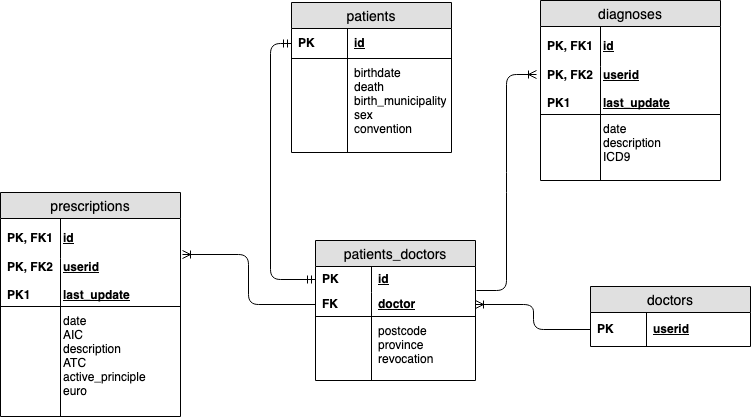
\includegraphics[scale=0.6]{images/er.png}
\end{figure}

